\documentclass[11pt, oneside]{article}   	% use "amsart" instead of "article" for AMSLaTeX format
\usepackage[margin=1in]{geometry}                		% See geometry.pdf to learn the layout options. There are lots.
\geometry{letterpaper}                   		% ... or a4paper or a5paper or ... 
%\geometry{landscape}                		% Activate for rotated page geometry
%\usepackage[parfill]{parskip}    		% Activate to begin paragraphs with an empty line rather than an indent
\usepackage{graphicx}				% Use pdf, png, jpg, or eps§ with pdflatex; use eps in DVI mode
								% TeX will automatically convert eps --> pdf in pdflatex		
\usepackage{amssymb}
%usepackage{undertilde}
\usepackage[numbered,framed]{matlab-prettifier}

\usepackage[T1]{fontenc}
\usepackage{mathtools}  % loads »amsmath«
\usepackage{physics}
\usepackage{listings}


\setlength{\parskip}{0.5em}
\lstset{
	language=C,                % choose the language of the code
	numbers=left,                   % where to put the line-numbers
	stepnumber=1,                   % the step between two line-numbers.        
	numbersep=5pt,                  % how far the line-numbers are from the code
	backgroundcolor=\color{white},  % choose the background color. You must add \usepackage{color}
	showspaces=false,               % show spaces adding particular underscores
	showstringspaces=false,         % underline spaces within strings
	showtabs=false,                 % show tabs within strings adding particular underscores
	tabsize=2,                      % sets default tabsize to 2 spaces
	captionpos=b,                   % sets the caption-position to bottom
	breaklines=true,                % sets automatic line breaking
	breakatwhitespace=true,         % sets if automatic breaks should only happen at whitespace
	title=\lstname,                 % show the filename of files included with \lstinputlisting;
}


%SetFonts
\newcommand\Rey{\mbox{\textit{Re}}}

\title{\vspace{-6ex} Assignment 3- Parallel Molecular Dynamics \\ {CSCI 596: Scientific Computing \& Visualization}  \vspace{-2ex}}
\author{Anup V Kanale}
\date{\vspace{-2ex}\today}							% Activate to display a given date or no date

\begin{document}
\maketitle \vspace{-5ex}

This purpose of this assignment is run molecular dynamics on multiple processors to understand asynchronous message passing and "in-situ" data analysis.
\vspace{-2ex} \section{Asynchronous Messages}
In this section, we use \texttt{MPI\_Irecv()} and \texttt{MPI\_Send()} with an \texttt{MPI\_Wait()} in the program \texttt{pmd.c}. The asynchronous messages make the deadlock-avoidance scheme unnecessary, and thus there is no need to use different orders of send and receive calls for even and odd-parity processes.

The new asynchronous implementation takes $5.13e-01$ seconds, whereas the original implementation takes $6.28e-01$ seconds. This observed speedup is $\approx 20\%$. The major modifications were made in the functions \texttt{atom\_copy} and \texttt{atom\_move}. To keep this report short, only these parts are shown in Appendix A.1.

\vspace{-2ex} \section{Communicators}
In this section, we basically allocate half the processors for the computations, and the other half for analysing the data from the computations. Specifically, following the lecture note on ``In situ analysis of molecular dynamics simulation data using communicators'', \texttt{pmd.c} is modified such that as many number of processes as that for MD simulations are spawned to calculate the probability density function (PDF) for the atomic velocity.

 The plot of the probability density function is as shown below:
 \begin{figure}[!htbp]
 	\centering
 	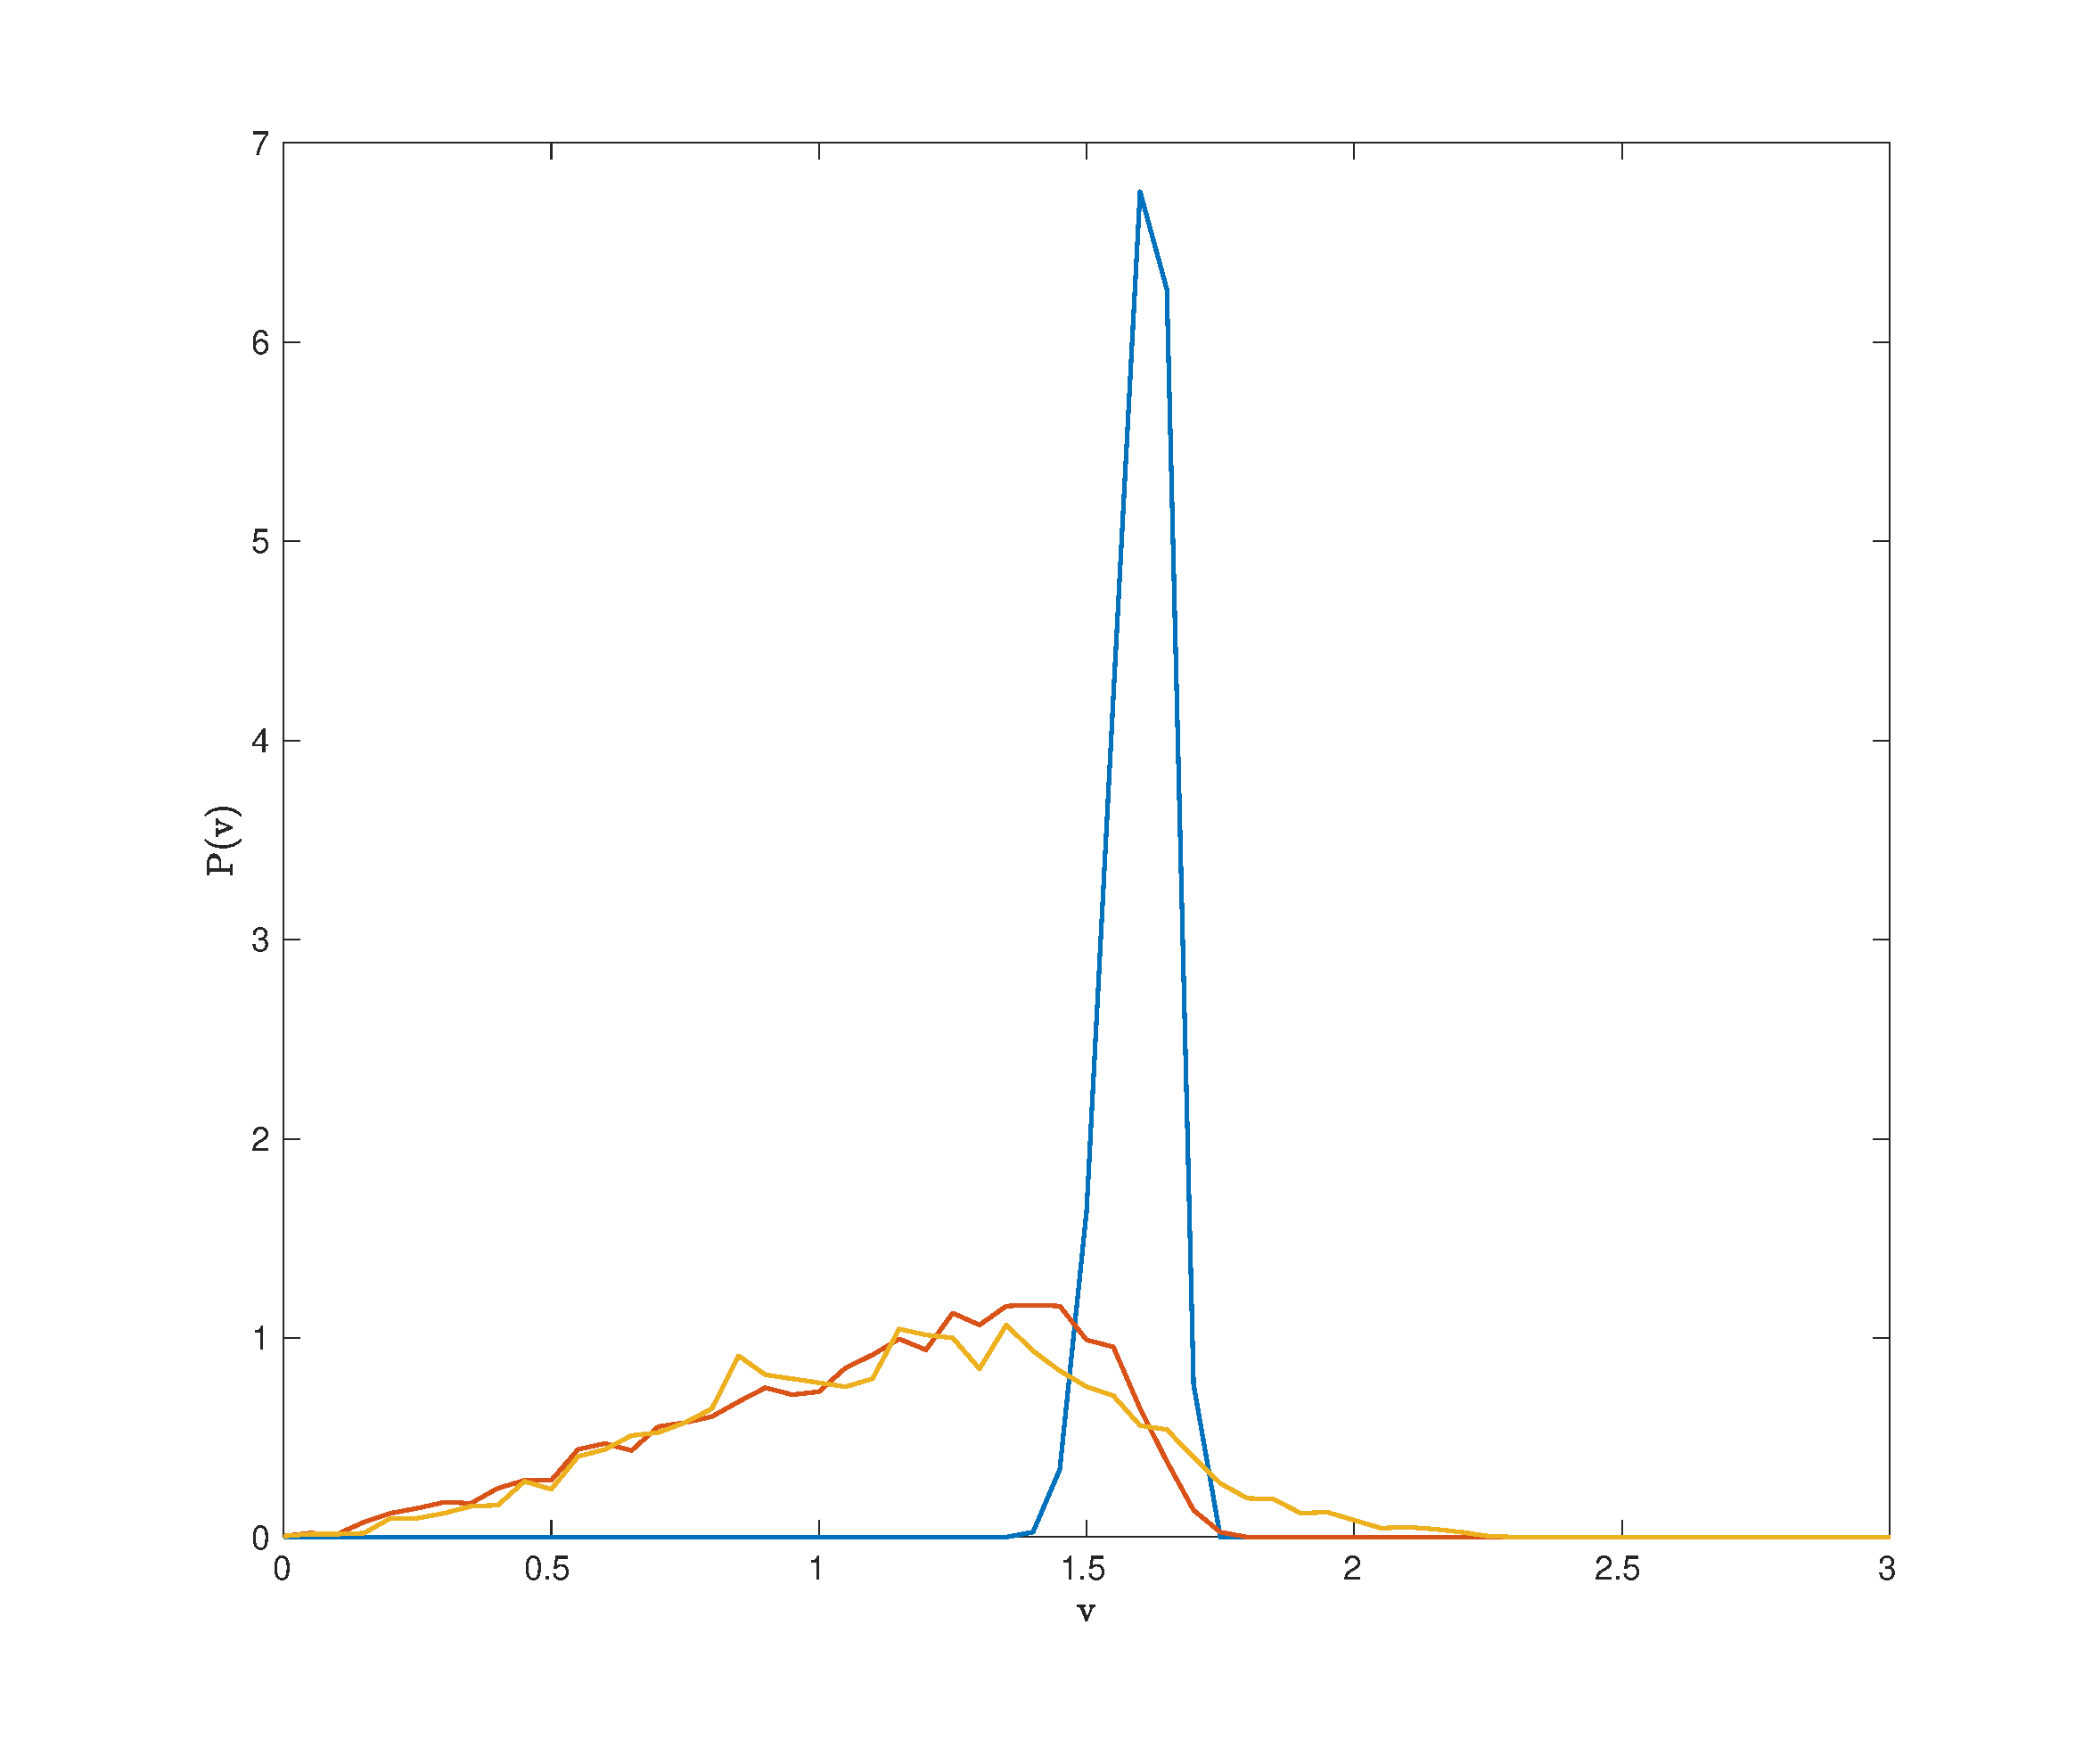
\includegraphics[scale=0.22]{probDensFunc.eps}
 	\caption{Probability density function}
 \end{figure}
The major modification was in the \texttt{main} function, \texttt{calc\_pv()} was provided. Only the modified portion is shown in appendix A.2 to keep this report short.

\appendix
\section{Appendix}
\subsection{Task I}
\lstinputlisting{pmd_async.c}

\subsection{Task II}
\lstinputlisting{pmd_async_task2.c}

\end{document}